%%%%%%%%%%%%%%%%%%%%%%%%%%%%%%%%%%%%%%%%%
% Short Sectioned Assignment
% LaTeX Template
% Version 1.0 (5/5/12)
%
% This template has been downloaded from:
% http://www.LaTeXTemplates.com
%
% Original author:
% Frits Wenneker (http://www.howtotex.com)
%
% License:
% CC BY-NC-SA 3.0 (http://creativecommons.org/licenses/by-nc-sa/3.0/)
%
%%%%%%%%%%%%%%%%%%%%%%%%%%%%%%%%%%%%%%%%%

%----------------------------------------------------------------------------------------
%	PACKAGES AND OTHER DOCUMENT CONFIGURATIONS
%----------------------------------------------------------------------------------------

\documentclass[paper=a4, fontsize=11pt]{scrartcl} % A4 paper and 11pt font size
\usepackage[shortlabels]{enumitem}
\usepackage{float}
\usepackage{ctex}
\usepackage{amssymb}
\usepackage{hyperref}
\usepackage{listings}
\usepackage[T1]{fontenc} % Use 8-bit encoding that has 256 glyphs
\usepackage{fourier} % Use the Adobe Utopia font for the document - comment this line to return to the LaTeX default
\usepackage[english]{babel} % English language/hyphenation
\usepackage{amsmath,amsfonts,amsthm} % Math packages

\usepackage{lipsum} % Used for inserting dummy 'Lorem ipsum' text into the template

\usepackage{sectsty} % Allows customizing section commands
%\allsectionsfont{\centering \normalfont\scshape} % Make all sections centered, the default font and small caps
\usepackage{mathrsfs}
\usepackage{fancyhdr} % Custom headers and footers
\usepackage{algorithm}
\usepackage[noend]{algpseudocode}
\algnewcommand\Break{\textbf{break}}

\usepackage{scrextend}
\usepackage{subcaption}
\graphicspath{{p3/}}
%\usepackage{algorithmic}
\usepackage[noend]{algpseudocode}
\usepackage{listings}
\pagestyle{fancyplain} % Makes all pages in the document conform to the custom headers and footers
\fancyhead{} % No page header - if you want one, create it in the same way as the footers below
\fancyfoot[L]{} % Empty left footer
\fancyfoot[C]{} % Empty center footer
\fancyfoot[R]{\thepage} % Page numbering for right footer
\renewcommand{\headrulewidth}{0pt} % Remove header underlines
\renewcommand{\footrulewidth}{0pt} % Remove footer underlines
\setlength{\headheight}{13.6pt} % Customize the height of the header

\numberwithin{equation}{section} % Number equations within sections (i.e. 1.1, 1.2, 2.1, 2.2 instead of 1, 2, 3, 4)
\numberwithin{figure}{section} % Number figures within sections (i.e. 1.1, 1.2, 2.1, 2.2 instead of 1, 2, 3, 4)
\numberwithin{table}{section} % Number tables within sections (i.e. 1.1, 1.2, 2.1, 2.2 instead of 1, 2, 3, 4)

\setlength\parindent{0pt} % Removes all indentation from paragraphs - comment this line for an assignment with lots of text

\newtheorem{theorem}{Theorem}[section]
\newtheorem{corollary}{Corollary}[theorem]
\newtheorem{lemma}[theorem]{Lemma}

%----------------------------------------------------------------------------------------
%	TITLE SECTION
%----------------------------------------------------------------------------------------

\newcommand{\horrule}[1]{\rule{\linewidth}{#1}} % Create horizontal rule command with 1 argument of height

\title{	
\normalfont \normalsize 
%\textsc{university, school or department name} \\ [25pt] % Your university, school and/or department name(s)
\horrule{0.5pt} \\[0.4cm] % Thin top horizontal rule
\huge Analysis and Design of Algorithm - Homework 6\\ % The assignment title
\horrule{2pt} \\[0.5cm] % Thick bottom horizontal rule
}

\author{宁雪妃} % Your name
%\author{Xuefei Ning} % Your name

\date{\normalsize\today} % Today's date or a custom date

\begin{document}

\maketitle % Print the title

%----------------------------------------------------------------------------------------
%	PROBLEM 1
%----------------------------------------------------------------------------------------

\section{Problem 1}
\textbf{16-2. 假定给定任务集合$S = {a_1, a_2, \dots, a_n}$, 其中任务$a_i$在启动后需要$p_i$个时间单位完成。你有一台计算机来运行这些任务, 每个时刻只能运行一个任务。令$c_i$表示任务$a_i$的完成时间, 即任务$a_i$被执行完的时间。你的目标是最小化平均完成时间, 即$\frac{1}{n}\sum_{i=1}^n {c_i}$。}

\begin{enumerate}[a]
\item \textbf{设计算法, 求平均完成时间最小的调度方案。任务的执行为非抢占式。证明算法能最小化平均完成时间, 并分析算法的运行时间。}
  %\begin{addmargin}[3em]{0em}
  
对于非抢占式, 没有释放时间规定的问题, 只需要将所有任务按照$p_i$从小到大排序, 然后按这个顺序调度即可。这个简单的算法可以最小化平均完成时间, 这是因为:

\begin{lemma}
  \label{lemma:1}
  对于任何一个任务子集$A \subseteq S$, 如果在调度$X$中, $a_n$在$a_m$之后被调度, 且$p_n < p_m$, 一定可以将$a_n$和$a_m$交换顺序得到一个新的调度$X'$, 使得该调度$X'$比$X$在平均完成时间上更优。
\end{lemma}
\begin{proof}
  假设$a_m$第$k$个被调度, $a_n$在$k + x$处被调度, $x > 0$。交换之前$A$中各个任务$a_i$的结束时间用$c_i$表示, $Cost(X) = \frac{1}{|A|}\sum_{a_i \in A} c_i$。那么将$a_n$和$a_m$任务交换次序后得到的新的调度$X'$的平均结束时间时间$Cost(X') = \frac{1}{|A|}\sum_{a_i \in A} c'_i$, 其中$c'_i$代表交换顺序后各个任务$a_i$的结束时间, 分为几种情况:
  \begin{itemize}
  \item 对于在$t < k$或者$t > k + x$的次序被调度的任务$a_i$, $c'_i = c_i$
  \item 对于在$k < t < k + x$次序被调度的任务$a_i$, $c'_i = c_i - (p_m - p_n) < c_i$
  \item 对于任务$a_m$, $c'_m = c_n$; 对于任务$a_n$, $c'_n = c_m - (p_m - p_n)$
  \end{itemize}
  所以$Cost(X') = Cost(X) - (p_m - p_n) \times x < Cost(X)$, 即$X'$比$X$在平均完成时间上更优。
\end{proof}

根据\hyperref[lemma:1]{该定理}, 可以知道拥有最优平均完成时间的调度一定是按照$p_i$从小到大的顺序调度任务$a_i$, 如果能找到一个逆序对, 一定可以交换两任务的调度顺序得到更优的调度。
%\end{addmargin}

\item \textbf{假定任务并不是在任意时刻都可以开始执行, 每个任务都有一个释放时间$r_i$, 在此时间之后才可以开始。此外假定任务执行是可以抢占的(preemption), 这样任务可以被挂起, 稍后再重新开始。设计算法, 对此问题求解平均完成时间最小的调度方案, 并证明算法确实能最小化完成时间, 分析算法的运行时间。}

  对于带释放时间的抢占式调度问题, 设计算法的时候, 我们观察到
  \[
  Cost(X) = \frac{1}{n} \sum_{i=1}^n c_i(X) = \frac{1}{n}\displaystyle\sum_{t=1}^{\sum_{i=1}^n p_i} {N_t(X)}
  \]
  其中$N_t$为$X$调度中在$t$时刻仍然没有执行完的任务数量。从这个式子的观察中, 我们知道: 在平均完成时间意义上最优的调度$X^{*}$中, 应该尽量让能够先执行完的任务尽快执行完, 使$N_t(X^{*})$尽量的小。由这个启发, 我们可以设计贪心算法如\hyperref[algo:1]{伪代码中}所示。

  \begin{algorithm}[H]
    \caption{MIN-AVG-FINISH-TIME-SCHEDULE($a$)}
    \label{algo:1}
    \begin{algorithmic}
      \State $n = \mbox{len}(a)$
      \State $X = []$
      \State $sort(a, \mbox{key}=\lambda (x): x.e)$ \Comment{将所有任务$a_i$按照$e_i$进行排序}
      \State $i = 0, j = 0$
      \State $H = \mbox{INIT-HEAP}(\mbox{key}=\lambda (x): x.p)$ \Comment{创建一个空的最小堆, 维护每个任务的剩余执行时间$a.p$的最小堆性质, $a_i.p$的初始值为$p_i$}
      \While{$i < n$}
      \State $j = i$
      \State $\mbox{cur\_time} = a[i].e$
      \While{$j < n \land a[j].e == a[i].e$}
      \State $\mbox{HEAP-INSERT}(H, a[i])$ \Comment{每个任务将被插入一次堆}
      \State $j+= 1$
      \EndWhile
      \If{$j >= n$}
      \While{$! \mbox{IS-EMPTY}(H)$}
      \State $\mbox{task} = \mbox{HEAP-EXTRACT-MIN}(H)$ \Comment{每个任务只会被从堆中删除一次}
      \State $X.\mbox{append}((\mbox{task}, \mbox{cur\_time}, \mbox{task}.p))$
      \EndWhile
      \State\Break
      \EndIf
      \State $\mbox{diff\_e} = a[j] - \mbox{cur\_time}$
      \While{$\mbox{diff\_e} != 0 \land !\mbox{IS-EMPTY}(H)$}
      \State $\mbox{task} = \mbox{HEAP-PEEK-MIN}(H)$ \Comment{$\Theta(1)$}
      \If $\mbox{task}.p > \mbox{diff\_e}$
      \State $\mbox{HEAP-DECREASE-KEY}(H, 0, \mbox{task}.p - \mbox{diff\_e})$ \Comment{只减小最小元素的$p$值, $\Theta(1)$}
      \State $X.\mbox{append}((\mbox{task}, \mbox{cur\_time}, \mbox{diff\_e}))$
      \State\Break
      \EndIf
      \State $\mbox{diff\_e} -= \mbox{task}.p$
      \State $\mbox{cur\_time} += \mbox{task}.p$
      \State $X.\mbox{append}((\mbox{task}, \mbox{cur\_time}, \mbox{task}.p))$
      \State $HEAP-EXTRACT-MIN{H}$ \Comment{$\Theta(\log(n))$, 每个任务只会被从堆中删除一次}
      \EndWhile
      \State $i = j$
      \EndWhile
      \State\Return $X$
    \end{algorithmic}
  \end{algorithm}

  这个算法返回的调度$X$为一个列表, 其中每个元素为一个三元组, 分别代表``任务'', ``开始执行时间'', ``持续执行时间''。按照开始执行时间顺序排列, 一个任务可能被挂起就可能在$X$列表中出现多次。从伪代码中可以看出这个算法中每个任务将被加入最小堆一次, 并从最小堆删除一次, 最坏情况下的复杂度为$\Theta(n\log(n))$。此外一开始需要对任务按照释放时间$e$进行排序, 需要$\Theta(n\log(n))$复杂度。总的算法复杂度为$\Theta(n\log(n))$。

  下面将证明该问题的贪心选择性质, 即一定可以在任意时间点选择已释放任务中剩余执行时间最小的任务来执行。
  \begin{lemma}
    \label{lemma:2}
    在任意单位时间片$t$, 如果某个已释放任务$a_i$需要的剩余执行时间$\hat{p}_i$是所有已释放任务中最小的, 那么该调度问题一定存在某个最优解, 在这个单位时间片$t$中执行$a_i$。
  \end{lemma}
  \begin{proof}
    如果存在某个最优解$X$, 其在时间片$t$选择了另一个已释放任务$a_j$来执行。我们可以构造调度$X'$, 构造方法如下:
    \begin{itemize}
    \item 如果在$X$调度中: $c_i \leq c_j$. 那么在$X$中将$t$时间片执行$a_i$, 并且让$X'$中$a_i$执行的最后一个时间片执行$a_j$。在这个新的调度$X'$中:
      \begin{itemize}
      \item $c'_k = c_k \quad k \neq i, j$: 除了$a_i$和$a_j$以外的其它任务$a_k$的终止时间$c_k$都不变。
      \item $c'_i = c_i - 1$
      \item $c'_j = \max(c_j, c_i) = c_j$
      \end{itemize}
      $Cost(X) - Cost(X') = c_i + c_j - c'_i - c'_j = 1 > 0$, 所以$X'$调度严格更优。
    \item 如果在$X$调度中: $c_j < c_i$. 那么将原来所有在$t$时间片以及$t$时间片以后执行$a_j$的前$p'_i$个时间片都换成执行$a_i$。并将原来$t$时间片以后的所有执行$a_i$的时间片都换成执行$a_j$。在这个新的调度$X'$中:
      \begin{itemize}
      \item $c'_k = c_k \quad k \neq i, j$: 除了$a_i$和$a_j$以外的其它任务$a_k$的终止时间$c_k$都不变。
      \item $c'_i < c_j$: 因为$\hat{p}_i < \hat{p}_j$, 所以$a_i$需要更少的时间片就可以执行结束。所以$a_i$在$X'$中的终止时间比$X$调度中任务$a_j$的终止时间要小。
      \item $c'_j = \max(c_j, c_i) = c_i$。
      \end{itemize}
      $Cost(X) - Cost(X') = c_i + c_j - c'_i - c'_j = c_j - c'_i > 0$, 所以$X'$调度严格更优。
    \end{itemize}
    综上, 只要不选择$a_i$作为$t$时间执行的任务, 就可以构造出$X'$比$X$更优。所以在任意时间点开始的子问题的最优解中, 在当前时间片一定选择执行已释放任务中剩余执行时间中最小的任务。
  \end{proof}

  最优子结构性质十分明显, 假设从$t$时间片开始的子问题$S_t$的调度为$X_t$, 因为$Cost(X_t) = Cost(X_{t+1}) + N_{t+1}/n$, 其中$N_{t+1}$是在第$t+1$个时间片开始时还没有执行完的任务数量。当选择做了之后, $N_{t+1}/n$是固定的: 所以当$S_t$得到最优解$X_t$时, 子问题$X_{t+1}$也必须是$S_{t+1}$的最优解, 否则可以将$S_{t+1}$的更优解$X'_{t+1}$直接替换得到一个更优的$S_t$问题的解$X'_t$。

  证明完了这两个性质, \hyperref[algo:1]{伪代码中所示算法}就是在每个时间片选择剩余时间最小的任务执行, 其中使用了$e_i$的信息进行了优化, 不需要在每个时间片都重新判断, 因为不是每个时间片都有新的任务被释放。只需要在有新任务被释放的时间片把新任务插入最小堆, 才需要做判断。
\end{enumerate}

\section{Problem 2}
\textbf{16-4. (调度问题变形) 对于带截止时间限制和惩罚的单位时间任务调度问题, 考虑如下算法。初始时令$n$个时间槽均为空, 时间槽$i$为单位时间长度, 结束于时刻$i$。按照惩罚值递减的顺序处理所有任务, 当处理任务$a_j$时, 如果存在不晚于$a_j$的截止时间$d_j$的空时间槽, 则将$a_j$分配到其中最晚的那个。如果不存在这样的时间槽, 将$a_j$分配到最晚的空时间槽。}

\begin{enumerate}[a]
\item \textbf{证明: 此算法总能得到最优解。}

  \begin{proof}
  书上已经证明``选择权重最大的提前完成的任务集合的问题''具有贪心选择性质和最优子结构性质, 题中所述的调度方法当然是合法的, 因为一个时间片只会调度一个任务。只要证明题中的判断方法也能选出``权重最大的提前完成任务的集合''即可。关键要证明题中的调度分配方法在每一次处理任务$a_j$时, 都正确的判断了$a_j$与之前选择的任务是否独立。如果题中的调度分配方法能够在每次处理任务$a_j \quad j = 0, 1, \dots, n$时都能正确的判断$a_j$和之前任务的独立性。则该问题能够得到一个正确的最优提前完成任务集合, 同时由于该问题调度方法是合法的(每个时间片只会调度一个任务, 且每个被选中提前完成的任务都被在它的截止时间之前完成), 该算法就能得到最优解。

  原始的独立性判据为:
  \[
  N_t(A) \leq t \quad \mbox{ for } t = 0,1, \dots, n
  \]
  其中$N_t(A)$为任务集合$A$中截止时间$d_i$在$t$之前的任务$a_i$的总个数。令
  \[
  \hat{N}_t(A) = \min_{k \geq t}{k - N_k(A)}
  \]
  $\hat{N}_t(A)$为每个时间位置$t$最多还能接受的$d_i = t$的任务$a_i$的个数, 该个数由所有$t$之后的时间点$k$是否均满足$N_k(A) \leq k$决定。
  \begin{corollary}
  由该定义式, 很显然对于任意一个集合$A$, 我们有$\hat{N}_{t+1}(A) \geq \hat{N}_t(A)$, 且大于和小于的情况:
  \begin{enumerate}[(I)]
  \item\label{corollary:em1} $\hat{N}_{t+1}(A) > \hat{N}_t(A)$: 只有当$t - N_t(A) < t + 1 - N_{t+1}(A)$时才可能成立, 即$N_{t+1}(A) < N_t(A) + 1$, 但是我们知道下式根据定义一定成立: $N_{t+1}(A) \geq N_t(A)$。所以此时一定有$N_{t+1}(A) = N_t(A)$(反之并不成立), 此时知道$\hat{N}_{t+1}(A) = \hat{N}_t(A) + 1$。
  \item $\hat{N}_{t+1}(A) = \hat{N}_t(A)$。
    %: 当$N_{t+1}(A) = N_t(A)$, 但又满足前面的式子时, 我们有
  \end{enumerate}
  \end{corollary}

  所以我们知道, 整个$1, 2, \dots, n$的截止时间区间可以根据递增的$\hat{N}_t(A)$值划分为多段, 每两段之间该值只差1, 每段里面该值相等。下面来考虑: 来了一个新的事件$a_j$时, 假设其截止时间为$d_j$, $d_j$落在$\hat{N}_t(A) = x$的段里。加入该事件后:
  \begin{itemize}
  \item 对于所有$t \geq d_j$的截止时间$t$: 由于对于所有的这些$t$, 都有新的$N'_t(A) = N_t(A) + 1$, 所以$\hat{N}'_t(A) = \hat{N}_t(A) - 1$。
  \item 对于在$\hat{N}_t(A) = x$的和$d_j$同一段的$t$, 且满足$t < d_j$的$t$: 由于$\hat{N}_t(A) = \min_{k \geq t}{k - N_k(A)}$, 而后面至少已经有一个$d_j$处的$d_j - N_{d_j}(A)$比原来小1了。可以知道对于这些$t$, 其对应的$\hat{N}'_t(A)$也都减去了1: $\hat{N}'_t(A) = \hat{N}_t(A) - 1$。
  \item 对于处于和$d_j$不同段且$t < d_j$的$t$, $\hat{N}_t(A) = \min_{k \geq t}{k - N_k(A)}$, 由于其本身的$N_t(A)$没有发生改变, 且由于$t$与$d_j$不同段, 根据前面的\hyperref[corollary:em1]{推导}, 我们知道一定有
    \[
    \min_{t \leq k < t_x} {k - N_{k}(k)} < \min_{k \geq t_x} {k - N_{k}(A)}
    \]
    其中$t_x$为所有和$d_j$同段中最小的$t$, 即$\min_{t \leq k < t_x} {k - N_{k}(k)} \leq \min_{k \geq t_x} {k - N_{k}(A)} - 1$。在加入$a_j$后, 后面的$k - N_{k}(A)$都只减小了1, 所以仍然满足$\min_{t \leq k < t_x} {k - N_{k}(k)} \leq \min_{k \geq t_x} {k - N_{k}(A)}$。所以对于这些$t$, $\hat{N}'_t(A) = \hat{N}_t(A)$, 并不改变。
  \end{itemize}

  可视化这个过程将更容易理解, 如\hyperref[fig:vis]{图}所示, 图中画出截止区间$t$的分段图。其中下标为0处的$\hat{N}_0(A)$肯定为0, 因为肯定不能接受任何一个$d_j = 0$的任务。如果加入一个$a_j$, 其$d_j = 7$, 分段图的变化如图所示: $d_j$属于$x = 3$一段, 找到这一段与上一段相接的边界, 将这个边界消去, 即可得到新的分段图。分段图上的$\hat{N}_t(A)$的具体值有所改变, 但那不是我们关注的重点, 我们只关心分段点在哪里即可。

  \begin{corollary}
    \label{corollary:2}
    到这里, 我们可以得到一个与原独立性判定方法完全等价的方法: 对于新加入的$a_j$任务, 从其截止时间$d_j$往前找到第一个分段点, 如果能够找到即说明加入该$a_j$任务后, 仍然满足独立性判据, 一定存在有某个调度可以使这个任务集合里的任务仍然都提前完成。
  \end{corollary}

  下面我们来证明题中的独立性判断方式跟\hyperref[corollary:2]{转化后的原判据}完全等价: 即题目中每一个空的时间槽$t \quad t = 1, 2, \dots, n$, 与\hyperref[corollary:2]{转化后判据}中的一个分段点$t - 1 <-> t$一一对应。这么明显的命题直接用归纳法进行证明即可:
  \begin{itemize}
  \item 最开始, 题目中所有的时间槽都为空, \hyperref[corollary:2]{转化后判据}中每个点都是分段点。
  \item 对于前面加入的任务该命题都成立, 现在加入一个新的任务$a_j$:
    \begin{itemize}
    \item 如果仍然满足独立性: 在\hyperref[corollary:2]{转化后判据}中, 从$d_j$开始往前找到的第一个分段点将被消除; 由归纳知该分段点对应题中方法的从$d_j$往前找的第一个空时间槽, 题中方法将填补该空时间槽。仍然保持一一对应关系。
    \item 如果不再满足独立性: 在\hyperref[corollary:2]{转化后判据}中, 从$d_j$开始往前找将找不到分段点, 与题中找不到空时间槽对应。此时题中算法将$a_j$放在最后一个非空时间槽将不影响任何其它任务的调度(显然, 相当于去掉了一个任务, 并且同时缩短了时间)。
    \end{itemize}
  \end{itemize}
  综上, 题中的算法可以找到最优调度。(好像证的有点麻烦, 主要是因为做作业之前自己思考了更优的解法, 顺序推理出了该转换, 然后该转换后的判定方法和题中的判定方法几乎一模一样, 所以干脆就用该转换作为中间判定方法来证明原判定和题中判定等价了。)
  \end{proof}

  \begin{figure}
    \centering
    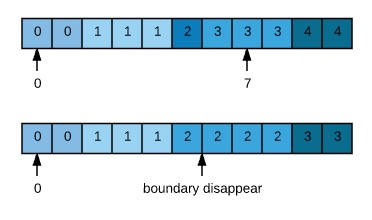
\includegraphics[height=32ex]{vis}
    \label{fig:vis}
  \end{figure}
\item \textbf{利用21.3节提出的快速不相交集合森林来高效实现此算法。假设输入任务集合已经按惩罚值单调递减的顺序排序。分析程序的运行时间。}
\end{enumerate}

\section{Problem 3}
\textbf{17.4-3. 假定改变表收缩的方式, 不是当装载因子小于$\frac{1}{4}$时将表规模减半, 而是当装载因子小于$\frac{1}{3}$时将表规模变成$\frac{2}{3}$。使用势函数:}
\[
\Phi(T) = | 2 T.\mbox{num} - T.\mbox{size} |
\]
\textbf{证明: 使用此策略, \textit{TABLE-DELETE}操作的摊还代价的上界是一个常数。}

\begin{proof}
  对于\textit{TABLE-DELETE}操作, 第$i$个操作用势能法写出的摊还代价为:
  \[
  \hat{c}_i = c_i + \Phi(T_i) - \Phi(T_{i-1})
  \]

  分类讨论:
  \begin{itemize}
  \item 当$\frac{1}{3} T.\mbox{size} \leq T.\mbox{num} \land T.\mbox{num} - 1 < \frac{1}{3}T.\mbox{size}$: \textit{TABLE-DELETE}操作会导致表收缩, 由于$\frac{1}{3}$将使得$\frac{1}{3}\mbox{size}$等数不再是整数, 为了严谨分类讨论:
    \begin{itemize}
    \item 当$T.\mbox{size}$为3的倍数时:
      \[
      \hat{c}_i = \frac{1}{3}T.\mbox{size} + (\frac{2}{3}T.\mbox{size} - 2(T.\mbox{num} - 1)) - (T.\mbox{size} - 2 T.\mbox{num}) = 2 = \Theta(1)
      \]
    \item 当$T.\mbox{size}$不为3的倍数时, 同样的有
      \[
    %\begin{split}
      \hat{c}_i = T.\mbox{size} - \lfloor \frac{2}{3} T.\mbox{size} \rfloor + (\lfloor \frac{2}{3}T.\mbox{size} \rfloor - 2(\lfloor \frac{1}{3}T.\mbox{size} \rfloor) - (T.\mbox{size} - 2 \lfloor \frac{1}{3}T.\mbox{size} + 1 \rfloor) = 2 = \Theta(1)
    %\end{split}
      \]
    \end{itemize}
  \item 当\textit{TABLE-DELETE}操作不导致表收缩时, 虽然存在$\frac{1}{2}T.\mbox{size}$这个势能函数的拐点, 但是统一的有: $\hat{c}_i = 1 + \Phi(T_i) - \Phi(T_{i-1}) = 1 + |T.\mbox{size} - 2 (T.\mbox{num} - 1)| - |T.\mbox{size} - 2 T.\mbox{num}| \leq 3$
  %% \item 当$\frac{1}{3} T.\mbox{size} < T.\mbox{num} \leq \frac{1}{2} T.\mbox{size}$: $\hat{c}_i = 1 + (T.\mbox{size} - 2(T.\mbox{num} - 1)) - (T.\mbox{size} - 2T.\mbox{num}) = 3 = \Theta(1)$
  %% \item 当$\frac{1}{2} T.\mbox{size} < T.\mbox{num} \leq T.\mbox{size}$: $\hat{c}_i = $
  \end{itemize}
  得证。
\end{proof}

\section{Problem 4}
\textbf{17-2. (动态二分查找) 有序数组上的二分查找花费对数时间, 但插入一个新元素的时间与数组规模成线性关系。我们可以通过维护多个有序数组来提高插入性能。}

\hspace{2em}\textbf{具体地, 假定我们希望支持$n$元集合上的\textit{SEARCH}和\textit{INSERT}操作。令$k = \lceil \log(n+1) \rceil$, 令$n$的二进制表示为$<n_{k-1}, n_{k-2}, \dots, n_0>$。我们维护$k$个有序数组$A_0, A_1, \dots, A_{k-1}$, 对$i = 0, 1, \dots, k-1$, 数组$A_i$的长度为$2^i$。每个数组或满或空, 取决于$n_i = 1$还是$n_i = 0$。因此, 所有$k$个数组里保存的元素总数为$\sum_{i=0}^{k-1} {n_i2^i} = n$。虽然单独每个数组都是有序的, 但不同数组中的元素之间不能存在特定的大小关系。}

\begin{enumerate}[a]
\item \textbf{设计算法, 实现这种数据结构上的\textit{SEARCH}操作, 分析其最坏情况运行时间。}

  假设为满的数组为$x$个, $x \leq k = \lceil \log(n+1) \rceil$。搜索元素$b$的算法描述如下:
  \begin{enumerate}
  \item 首先对每个为满的数组$A_i$, 以它们的数组头构建最小堆。花费$\Theta(x)$的时间。
  \item 循环: $\Theta(1)$查看堆中最小的元素$a$:
    \begin{itemize}
    \item 如果$a == b$, 则找到对应元素, 结束搜索循环;
    \item 若$b < a$, 则$b$不存在, 结束搜索循环;
    \item 若$b > a$, 继续循环:
      \begin{itemize}
      \item 如果$a$所在的数组还有其它元素, 将$a$所在数组的下一个元素代替$a$的位置, 并调用$\mbox{MIN-HEAPIFY}$。花费$\Theta(\log(x))$;
      \item 如果$a$所在的数组没有其它元素, 直接调用$\mbox{HEAP-DELETE}$。花费$\Theta(\log(x))$;
      \end{itemize}
    \end{itemize}
  \end{enumerate}
  最坏情况下$x = k = \lceil \log(n+1) \rceil$, 且$b$比数据结构中最大的数还要大, 此时搜索需要耗时$\Theta(n \log(n))$。

\item \textbf{设计\textit{INSERT}算法。分析最坏情况运行时间和摊还时间。}

  \textit{INSERT}算法插入元素$b$的步骤如下:
  \begin{enumerate}
  \item 创建一个新数组$A_0$只包含要插入的元素$b$。$\Theta(1)$
  \item 找到第一个满足$A_i$为空的数组下标$i$。$O(n)$
  \item 对于$A_0, \dots, A_{i-1}$的数组实现最小堆归并排序, 构成新的$A_{i}$。并且释放$A_0, \dots, A_{i-1}$的空间。$\Theta(2^i\log(i))$
  \end{enumerate}

  上面算法描述中的归并排序方法与\textit{SEARCH}算法中所使用的一样, 通过构建最小堆实现, 具体见\textit{SEARCH}算法的描述。

  最坏情况下, 运行时间为$\Theta(n\log(n))$。

  考虑$n$次插入操作, 每个$A_i \quad i = 0, \dots, k-1$从空变成满的次数为$n/2^{i+1}$次, 每次$A_i$从空变成满所花时间为$\Theta(2^i\log(i+1))$, 摊还时间为:
  \[
  \begin{split}
    \Theta(\frac{1}{n}\displaystyle\sum_{i=1}^{k} \frac{n}{2^{i+1}} 2^i \log{i}) = \Theta(\displaystyle\sum_{i=0}^{k} \log(i)) = \\
    \Theta(k\log(k)) = \Theta(\log(n)\log(\log(n)))
  \end{split}
  \]
  其中后一步推导可以利用黎曼积分的定义, 给求和式算出积分上下界, 即可简单推出。这里不再赘述。

  即插入操作的摊还时间为$\Theta(\log(n)\log(\log(n)))$。

\item \textbf{讨论如何实现\textit{DELETE}。}

  要\textit{DELETE}某个元素$b$:
  \begin{enumerate}
  \item 先使用\textit{SEARCH}算法找到$b$元素在数据结构中对应的元素$a = b$的位置, 假设为$A_i$数组中的第$k$号元素。最坏情况下$\Theta(n \log(n))$
  \item 假设现在最小的满足$A_j$为满的下标为$j$:
      \begin{itemize}
      \item 如果$i = j$: 直接从$A_i$中删除$a$元素, 并把$A_i$数组剩下的元素顺序切分为元素个数分别为$1, \dots, 2^m, \dots, 2^{i-1} \quad m = 0, \dots, i-1$的数组, 并依次赋值给$A_0, \dots, A_{i-1}$即可。复杂度$\Theta(2^j)$。
      \item 否则: 将$A_j$当前在最小堆中的元素$a_j$插入$A_i$数组, 并移除$A_i$数组中的$a$元素。$a_j$元素满足$a_j > a$, 所以只要在$A_i$的$a$元素后做二分查找查找到应该要插入的位置$k'$, 即可插入。插入操作还需要$k' - k$的复杂度, 所以最坏情况下这步操作的复杂度为$\Theta(2^i)$。然后继续对$A_j$进行拆分操作, 复杂度$\Theta(2^j)$。
      \end{itemize}
      这步在最坏情况下的复杂度为$\Theta(2^i)$。
  \end{enumerate}

  最坏情况下是$\Theta(n\log(n))$的复杂度。
\end{enumerate}

\end{document}
